\documentclass{article}
\usepackage{amsmath, amssymb, amsthm, graphicx}
\newtheorem{theorem}{Theorem}
\renewcommand{\refname}{Bibliography}
\begin{document}
	\begin{titlepage}
		\title{Improvements to the immersiveness  of motion controls for video games}
		\date{April 10, 2017}
		\author{T. Maxwell Thomas and David Darrow}
		\maketitle
	\end{titlepage}
	\section{Abstract}
	
	This report details the results of a project to develop an improved motion controller for video games in the form of a glove which translates the hand and arm movements of the user into commands for a connected computer. Described are existing technologies and their shortcomings, technical details of the glove's function, and results of experimental testing of the glove.
	\section{Background}
	
	The games industry has produced several motion control schemes, each with its own shortcomings that the glove is designed to address. More traditional motion controls, such as those for the Nintendo Wii, only provide the ability to move the controller as an aid to immersion-the user is still required to press buttons in order to trigger actions. Furthermore, traditional motion controls require that the games they are used for be designed specifically with the controllers in mind-something uncommon in recent games, but impossible for older titles developed before motion controls were released.
	
	Another form of control is the full-on virtual reality system, such as the HTC Vive. These systems, while impressive pieces of technology, come with their own set of problems. They require a substantial open area in order to function properly, something not necessarily available to users. They're quite expensive, and they still require button presses---and support from games in order to be used.
	
	The glove is designed to provide user-customizable controls based on both broad and fine hand and arm movements, with the intention of providing a more natural control input scheme than is afforded by any other input system. Unfortunately, this is unlikely to prove a suitable replacement for existing motion control schemes because the motions take too long for high-precision play, and the variety of motions one could reasonably be expected to contend with does not provide sufficient controls for many games. Rather, the glove is intended as a proof-of-concept and novelty item, demonstrating the possibility of such technology. Developing a proper commercial product is beyond the budget and scope of this project, as well as the skills of the authors.
	
	This isn't the first time a group has attempted to make a glove-shaped motion controller. The general concept, called a wired glove, dates back to 1977 with the Sayre glove. The first motion-sensing glove to be applied to the purposes of video game control was the Nintendo Power Glove, released in 1989. The Power Glove was designed as a derivative of the VPL DataGlove, modified to decrease the cost in order to make the glove accessible to a broad consumer market. However, this glove only met with limited success due to being both clumsy and uncomfortable to wear. Dissuaded by the lack of success of the Power Glove, especially considering the measures taken to make it a practical prospect, companies transitioned their efforts to designing more traditional controllers with integrated inertial positioning, leaving wired glove technology by the wayside.
	
	There are two ways in which the glove described in this report differs from prior wired gloves. Firstly, prior gloves focused on detecting individual joint bending via flex sensors. Our glove, however, only records fingertip positions for the thumb, index finger, and middle finger, since their position and motion is contingent on the movements of the rest of the hand (the ring and pinky fingers do not readily move independent of the middle and index fingers). Secondly, past gloves have kept track of the position of the glove via dead reckoning from the sensor readings collected. While this may be desirable in full virtual-reality simulations or other similar applications, it's unnecessary when we're trying to simply compare user hand motions to recorded ones. We instead compare acceleration curves.
	
	\section{Design specifics \& potential alternatives}
	\subsection*{Glove Electronics}
	
	The glove uses two dedicated 3-axis MMA8451 accelerometers on the thumb and middle fingers, and a 3-axis LSM303 combined accelerometer/magnetometer for reading the glove's current trajectory. Data from the sensors is transmitted ten times per second to a glove-mounted microcontroller over an I\textsuperscript{2}C bus, and then over a serial line transmitting at 9600 baud to the connected computer. Due to the glove's low on-board processing power, and lack of long-term storage for anything other than the program, the task of translating glove movements to controls and recording target motions for later use is entirely that of the computer the glove is connected to. 
	
	The glove itself is a Kevlar work glove, picked for the durability of the material. The wires are sewn directly into the glove and coated with an insulating resin to prevent shorts between the bare wires. Graph theory was used to determine a layout for the wires that had no branching paths or crossed wires, to enable the wires to be sewn into the glove. \newline
	
	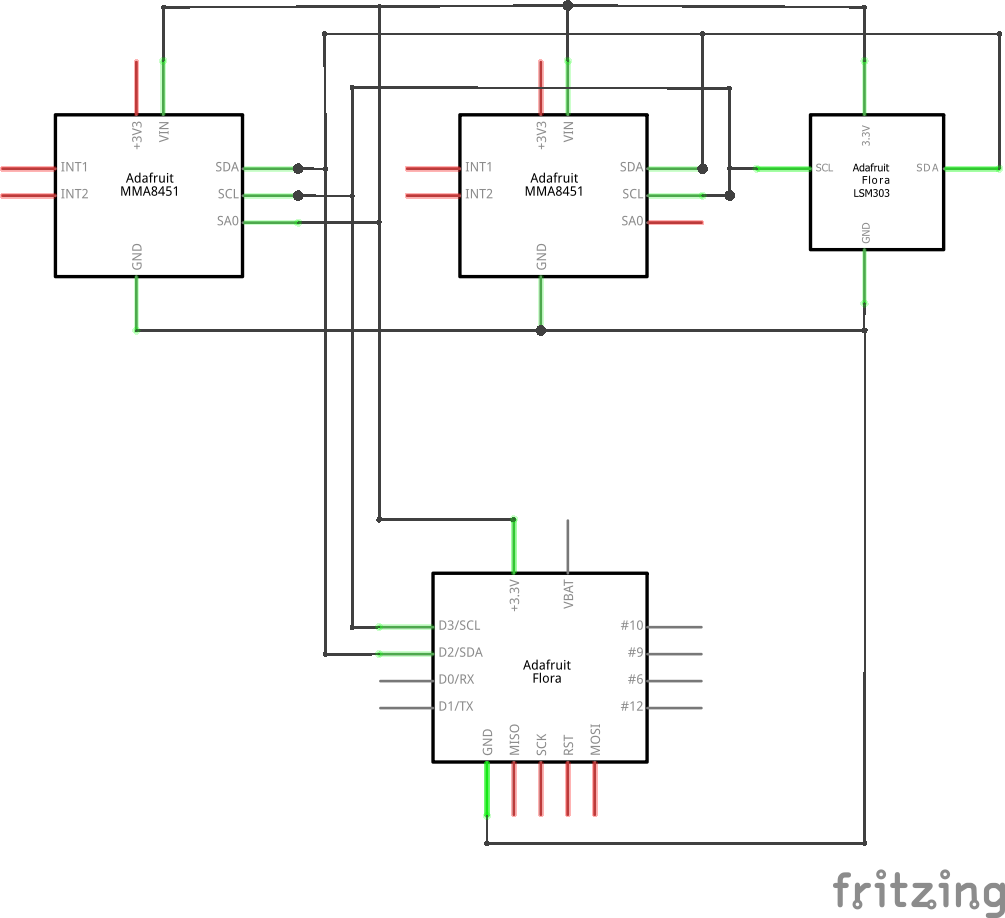
\includegraphics{Glove_schematic}
	\newline
	\begin{center}
		\textit{Figure 1: Glove electrical schematic}
	\end{center}
	\subsection*{Computer I/O and Interface}
	
	The computer receives data from the glove in 4-byte packages, with each package representing one of the 12 floating-point values that represent the acceleration and orientation detected by the sensors on the glove. These values are then stored in a temporary buffer, and either written to a file in the case of macro creation, or compared to recorded macros loaded for a file in the case of macro execution. The glove sends updated sensor readings to the computer every fifth of a second, with the incoming messages from the glove (which synchronizes off of its internal clock) taking care of program timing for the computer. The computer program is split into two executables---one for recording macros, and one for comparing glove movements to recorded macros and executing when necessary. The macros themselves are stored in user-specified files, permitting several different combinations of controls.
	
	Both executables are written strictly for Linux (the end user's operating system), and run purely off of the terminal. Note that, while terminal applications can be cross-platform, this one is not; this is due to both use of X11 calls to simulate keystrokes and due to the particular way Unix-based operating systems handle serial ports.
	\subsection*{Macro Detection Algorithm}
	
	Here is a simple algorithm for error analysis in $\mathbb{R}^n$, using approximate integration in place of scaled sum-of-squares methods, to compare two functions $f_0(t)$ and $f(t)$. The two functions are sampled $N$ times at equidistant points in the interval $t\in[0,1]$.
	
	Let $(t_i)_0^{N-1}$ be points equally spaced in the interval $t\in[0,1)$, such that $t_k-t_{k-1}=\frac{1}{N}$ for all $k>1$ and $t_1=0$. Define $t_{N}=1$. 
	
	The \emph{sum-of-squares} method measures the square of the distance between vectors in $\mathbb{R}^n$. Calling the output "error" $e$ and the initial vector (to be compared to), it can be described as follows:
	
	\begin{equation} e \approx \frac{1}{N}\sum\limits_{k=0}^{N-1} [f(t_k)-f_0(t_k)]^2 .\end{equation}
	
	This can be seen as a "left-hand" Riemann sum of $N$ terms to approximate the corresponding Riemann integral,
	
	$$e \equiv \int_0^1 [f(k)-f_0(k)]^2\;dk.$$
	
	To better approximate this integral, we use a \emph{cubic spline interpolant}. To do this, we need $f_0(t)$, $f(t)$, $\frac{d}{dt}f_0(t)=f_0'(t)$, and $f'(t)$ sampled at $(t_k)_0^N$.
	
	\begin{theorem}
		There is a unique cubic polynomial $P$ that solves the following set of equalities:
		$$P_j(0)=[(f-f_0)(t_j)]^2$$
		$$P_j(1)=[(f-f_0)(t_{j+1})]^2$$
		$$P_j'(0)=\frac{1}{N}\frac{d}{dt_j}[(f-f_0)(t_j)]^2=\frac{2}{N}[(f-f_0)(t_j)][(f'-f'_0)(t_j)]$$
		$$P_j'(1)=\frac{1}{N}\frac{d}{dt_{j+1}}[(f-f_0)(t_{j+1})]^2=\frac{2}{N}[(f-f_0)(t_{j+1})][(f'-f'_0)(t_{j+1})].$$
		
		This polynomial is given by 
		$$P_j(x)=P(0)(1-3x^2+2x^3)+P(1)(3x^2-2x^3)+P'(0)(x-2x^2+x^3)+P'(1)(-x^2+x^3).$$
	\end{theorem}
	
	\begin{proof}
		Define 
		$$Q(x)=a(1-3x^2+2x^3)+b(3x^2-2x^3)+c(x-2x^2+x^3)+d(-x^2+x^3).$$
		
		Evaluating, taking derivatives, and evaluating again, it clearly solves the equalities $Q(0)=a$, $Q(1)=b$, $Q'(0)=c$, and $Q'(1)=d$. 
		
		To prove uniqueness, assume some $Q_0$ solves the same equalities. Then $(Q-Q_0)(0)=(Q-Q_0)(1)=0$. From little B\'{e}zout's Theorem, $(Q-Q_0)(x)=px(x-1)(x-q)$, so $0=(Q'-Q'_0)(0)=pq$ and $0=(Q'-Q'_0)(1)=p(1-q)$. So, $0=p(1-q)+pq=p$ and $Q=Q_0$.
		
		Set $$(a,b,c,d)=$$
		$$\big([(f-f_0)(t_j)]^2,[(f-f_0)(t_{j+1})]^2,\frac{1}{N}\frac{d}{dt_j}[(f-f_0)(t_j)]^2,\frac{1}{N}\frac{d}{dt_{j+1}}[(f-f_0)(t_{j+1})]^2\big)$$
		
		to obtain $P_j(x)$, as in the hypothesis of this theorem.
	\end{proof}

	We then map $[t_k,t_k +\frac{1}{N})$ to $[0,1)$ with the affine transformation 
	
	$$A_k(t)=N(t-t_k).$$
	
	By defining a function $P(x)=\{(P_k\circ A_k)(x) \; | x \in [t_k,t_{k+1}], \;0\leq k \leq N \}$, we obtain a $C^2$ interpolant to $[(f-f_0)(x)]^2$ over the half-open interval $[0,1)$. We integrate piecewise over each $(P_k\circ A_k)$, obtaining the identity

	$$ e \equiv \int_0^1 [f(k)-f_0(k)]^2\;dk \approx$$
	\begin{equation}\frac{1}{2N}[(f-f_0)(0)]^2+\frac{1}{2N}[(f-f_0)(1)]^2+\frac{1}{N}\sum\limits_{k=1}^{N-1} [(f-f_0)(t_k)]^2 + \end{equation}
	$$ \frac{1}{6N^2}[(f-f_0)(0)][(f'-f'_0)(0)] - \frac{1}{6N^2}[(f-f_0)(1)][(f'-f'_0)(1)] .$$
	
	Thus we obtain a second order error approximation without requiring much additional information. This is applied to our glove by replacing $N$ with $\llcorner TN \lrcorner$, where $T$ is the time taken by a macro. Each macro then stores start and end derivatives, as well as values at each $t_k$; at each time step, we compare our data $f$ to our macro $f_0$.
	
	Failing direct calculation of $f'$, we approximate it using appropriate high-order finite difference methods.
	
	\subsection*{Potential alternatives}
	
	Possible alternatives for the design include using optical position sensors to accurately locate the glove, using a gyroscope instead of a magnetometer for detection of orientation, and using a custom circuit to feed data to the host computer instead of using a microcontroller. Each of these was rejected, for the following reasons:
	
	The optical position sensors, while in every way a more optimal solution to the problem, were well beyond both the means and the skills of the project team to create or use. Furthermore, they would have added additional necessary devices, a suboptimal solution for what was intended to be a standalone device.
	
	A gyroscope would have been less susceptible to interference. However, gyroscopes are subject to drift even over relatively short timeframes, while magnetometers, orienting based on Earth's magnetic field, are not. This is especially true at the commercial level, at which this project is operating. Furthermore, we were able to find an off-the-shelf accelerometer/magnetometer, while no combined accelerometer/gyroscope appeared to be available.
	
	The thought of using a custom chip instead of a microcontroller may have made sense at the commercial level, but for an individual project like this one it was much simpler to just take a microcontroller and program it to do whatever we required of it. Printing circuits is expensive, especially circuits as complicated as would have been necessary, had we tried to make a custom board. In sum, using the microcontroller made more sense because of the low cost, ready availability, and the fact that they allow for rapid prototyping due to the dynamic nature of the system.
	
	
	\section{Results}
	
	
	Unfortunately, due to an inexplicable malfunction in the glove's microprocessor that caused it to stop responding to all input (including the on-board reset button), we were never able to fully test the glove's features. However, the serial communication capabilities of the microcontroller (or one like it) were confirmed to support the necessary transmission rates, and the algorithm for macro recognition functioned as desired.
	
	Further work could make the glove function, although there may be problems with the wiring that will prove difficult to fix. The mathematics, however, will almost certainly function as intended. Even if initial tests prove precise motion replication to be too difficult, it's trivial to increase the error tolerance and alleviate the problem.
	
	\section{Conclusion}
	
	While the concept of a motion-detecting glove seems workable in theory, and all necessary components were developed to one extent or another, it has so far been non-functional in practice. Moreover, it's likely the glove would never have worked as intended, even if it could have been made to function as well as possible. This is because of latency between actions performed and actions executed-the time it takes to perform a meaningful hand motion- is often too long to permit accurate control, especially considering that any controls executed will only occur after the motion has been finished. Unfortunately, to achieve real-time control would require support built into whatever game one is trying to play-which partially defeats the point of the glove. \newpage
	
	\begin{thebibliography}{9}
		\bibitem{mma8451}
		Freescale Semiconductor, \text{"3-Axis, 14-bit/8-bit digital accelerometer"}, MMA8451q datasheet, Feb. 2017 (rev. 8)
		
		\bibitem{littlethm}
		P. Rudnicki, "Little Bezout Theorem (Factor Theorem)" in 
		\textit{Formalized Mathematics vol. 12},
		R. Matuszewski, G. Bancerek, and P. N. Kawamoto, Eds., 
		Berlin: Walter de Grutyer, 2004, pp-49-58.
		
		\bibitem{lsm303}
		STMicroelectronics, "Ultra compact high performance e-compass 3D accelerometer and 3D magnetometer module", LSM303DLHC datasheet, Apr. 2011 (rev. 1)
		
		\bibitem{ieee:cga}
		D. J. Sturman and D. Zeltzer, "A Survey of Glove-based Input", 
		\textit{IEEE Computer Graphics and Applications}, vol. 14, no. 1, Jan., pp. 30-39, 1994.
		
		\bibitem{chfcs:hjid}
		T. G. Zimmerman et al., "A Hand Gesture Interface Device."
		\textit{Proceedings of the SIGCHI/GI Conference on Human Factors in Computing Systems and Graphics Interface}, ACM Press, New York, April 1987, pp 189-192
	\end{thebibliography}
\end{document}